\documentclass{article}
\usepackage[margin=2cm]{geometry}
\usepackage{graphicx}
\usepackage[pages=some]{background}
\usepackage{titling}
\usepackage{tabularx}
\usepackage{tikz}
\usepackage{forest}
\usepackage{float}
\usepackage{amsmath}
\usepackage{amssymb}
\usepackage{xcolor}
\usepackage{tcolorbox}
\usepackage{multicol}

\forestset{
  my box/.style={
    draw,
    rectangle,
    rounded corners,
    fill=gray!20,
    inner sep=6pt,
    minimum width=3cm % Adjust the width as needed
  }
}


\geometry{a4paper}

\backgroundsetup{
    scale=1,
    angle=0,
    opacity=1,
    contents={%
        
\includegraphics[width=\paperwidth,height=\paperheight]{institution_logo.jpg}
    }
}

\newcommand{\subtitle}[1]{
    \posttitle{
        \par\end{center}
        \begin{center}\large#1\end{center}
        \vskip0.5em}
}

\title{ME-421}
\author{Md. Hasibul Islam}
\subtitle{FLUID MACHINERY}

\begin{document}
\begin{titlepage}
    \centering
    
    {\Huge\bfseries\maketitle}
    \textbf{Mohammad Ali Sir} \\
    \vspace{2cm}
    
\includegraphics[width=8cm]{institution_logo.jpg}
    \vfill
    \vspace*{2cm}
\end{titlepage}

\tableofcontents
\pagebreak
\section{Lecture 01: Introduction} 
\hfill Date: 03/06/2023
\subsection*{Booklist}

\textbf{Hydraulic Machines through worked out problems}

\hfill Published by BUET


\section{Lecture 2: Principles of Hydraulic Machinery}
\hfill Date: 05/06/2023

\subsection{Dynamic Action of Fluid}

When a stream of fluid enters a machine, it generally follows a specific direction. However, in order to alter its velocity, either in magnitude or direction, a force must be applied to the fluid. This force, exerted by the motion of the fluid, is referred to as dynamic force. The power of the machine is determined by the dynamic force generated by the flowing fluid, which arises due to the change in momentum.

Momentum can exist in linear or angular form, with angular momentum being the moment of linear momentum. The force is the rate of change of linear momentum, while torque is the rate of change of angular momentum. According to Newton's second law, the rate of change of momentum is proportional to the applied force and occurs in the direction of the force. Specifically, if the resultant external force in the $x$-direction is $F_x$, the mass of the fluid is $m$, the velocity of the fluid is $v_x$, and the change in velocity over time $dt$ is $dv_x$, then:
\\

The change in momentum = $mdv_x$,

And the rate of change of momentum  $= m \frac{dv_x}{dt}$
\begin{equation}
F_x = m \frac{dv_x}{dt} \label{eq:eq1}
\end{equation}

$eq^n$ (\ref{eq:eq1}) is knows as linear momentum $eq^n$.

This $eq^n$ may be wriiten as -
\begin{equation}
F_x dt = mdv_x \label{eq:eq2}
\end{equation}

This $eq^n$ is known as impulse momentum $eq^n$.

For a control volume with fluid entering in uniform velocity $v_{x_{1}}$, and leaving after time $t$ within uniform velocity $v_{x_{2}}$, then according to $eq^n$ (\ref{eq:eq2}),
\begin{equation}
	F_x = \frac{m}{t} (v_{x_{2}}-v_{x_{1}}) \label{eq:eq3}
\end{equation}

Again, $$\frac{m}{t}=\rho Q$$
\begin{equation}
	\Rightarrow F_x = \rho Q (v_{x_{2}}-v_{x_{1}}) \label{eq:eq4}
\end{equation}

Dynamic force exerted by fluid jet on stationary flat plate - 

\subsubsection{Plate normal to jet:}
A fluid jet is issued from a nozzle and strike a flat plate with a velocity $v$. The plate is held stationary at perpendicular to the centerline of the jet. Let,

\begin{center}

$Q \longrightarrow $  Volumetric flow rate\\
$\rho Q \longrightarrow$ Mass flow rate
\end{center}

Dynamic force on the fluid by the plate:
\\
Applying $eq^n$ \ref{eq:eq4}, 
$$F_x = \rho Q (v_{x_{2}} - v_{x_{1}}) $$
$$\Rightarrow -F_x = \rho Q (0-v)$$
\begin{equation}
	\Rightarrow F_x = \rho Q v \label{eq:eq5}
\end{equation}
\begin{equation}
	\Rightarrow F_x = \frac{\gamma}{g} Q v \label{eq:eq6}
\end{equation}

\begin{figure}[H]
  \centering
  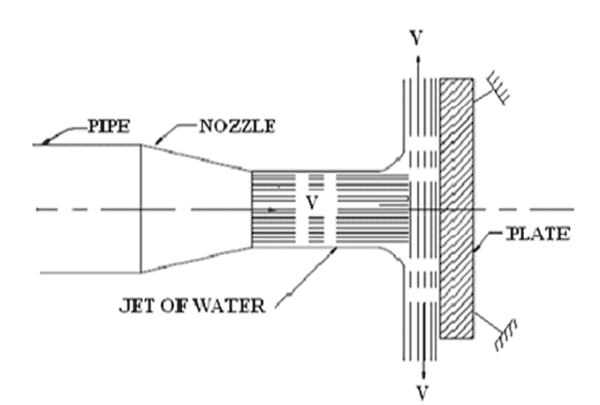
\includegraphics[width=0.75\textwidth]{img/flat_plate.png}
  \caption{Plate normal to jet.}
  \label{fig:Plate normal to jet}
\end{figure}

If $a$ is the area of jet,
$$F_x = \frac{\rho}{g} a v  v$$
\begin{equation}
	\textcolor{red}{\Rightarrow F_x = \frac{\rho}{g} a v^2} \label{eq:eq7}
\end{equation}

\subsubsection{Inclined Plate}
\begin{figure}[H]
  \centering
  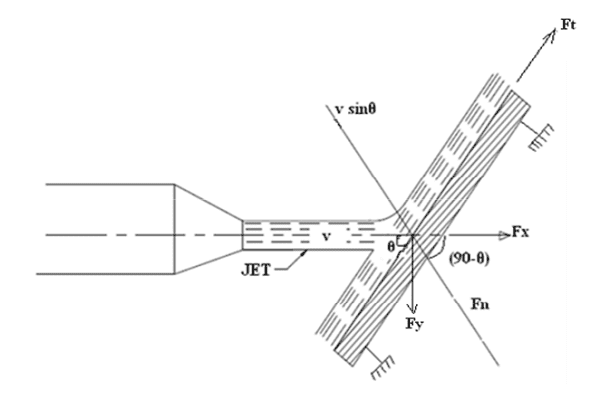
\includegraphics[width=0.75\textwidth]{img/inclined_plate.png}
  \caption{Plate inclined to jet.}
  \label{fig:Plate inclined to jet}
\end{figure}
\vspace{0.25cm}

$$F = F_n = \rho Q v sin\theta $$
Again, $$F_x = F sin\theta$$
$$= (\rho Q v sin \theta) sin \theta $$
\begin{equation}
	\textcolor{red}{F_x = \rho Q v sin^2 \theta} \label{eq:eq8}
\end{equation}
\\
And, $$F_y = F cos\theta$$
\begin{equation}
	\textcolor{red}{\Rightarrow F_y = \rho Q v sin\theta cos\theta} \label{eq:eq9}
\end{equation}
\vspace{0.25cm}
\paragraph*{Determine of division of flows:}
Let $F_s$ ($F_t$ in fig. \ref{fig:Plate inclined to jet}) be the force along the inclined surface of plate and $Q_1$ and $Q_2$ are quantities of flow along the surface. As there is no change in elevation of pressure before and after impact, the magnitude velocity leaving the plate will remain the same. \\
\\
since no force is exerted on the fluid by the plate in "S" direction, then,
\begin{equation}
	F_s = 0 = \rho Q V cos\theta \label{eq:eq10}
\end{equation}
Again, 
\begin{equation}
	\rho Q_1 v - \rho Q_2 v = 0 \label{eq:eq11}
\end{equation}

From $eq^n$ (10) \& (11),
$$\rho Q v cos\theta = \rho Q_1 v - \rho Q_2 v $$
\begin{equation}
	\Rightarrow Q cos\theta = Q_1 - Q_2 \label{eq:eq12}
\end{equation}

From continuity $eq^n$, 
\begin{equation}
	Q_1 + Q_2 = Q \label{eq:eq13}
\end{equation}

From $eq^n$ (12) \& (13),


$$Q_1 = \frac{1}{2} Q (1+cos\theta)$$ 
  \begin{equation}
     Q_2 = \frac{1}{2} Q (1-cos\theta) \label{eq:eq14} 
  \end{equation}

\pagebreak

\section{Lecture 3}
\hfill Date: 12/06/2023

\subsubsection*{Problem}
A jet of water with a velocity of 35 $m/s$ strikes a plat inclined of 30°, cross sectional area if jet 25 $cm^2$. Find the force exerted by the jet on the plate. Calculate the components of force and find the ratio in which the discharge gets divided after striking the plate. 

\subsubsection*{Solution:}
Given, 
\begin{align*}
  \text{velocity, } v &= 35 \, \text{m/s}\\
  \text{angle, } \theta &= 30^\circ \\
  \text{cross-sectional area, } a &= 25 \, \text{cm}^2 \\
  \\
  \text{Volumetric flow rate, } Q &= a \times v \\
  &= 0.0025 \times 35 \, \text{m}^3/\text{s} \\
  &= 0.0875 \, \text{m}^3/\text{s} \\ 
  \\
  \text{Force, } F &= \rho Q v \sin\theta \\
  &= 1000 \times 0.0875 \times 35 \times \sin(30^\circ) = 1531.25 \, \text{N} \\
  \\
  F_x &= F \sin\theta = 765.6 \, \text{N} \\
  F_y &= F \cos\theta = 1326.1 \, \text{N} \\
  \\
  Q_1 &= \frac{Q}{2} (1 + \cos\theta) = 0.0816 \, \text{m}^3/\text{s}\\
  Q_2 &= \frac{Q}{2} (1 - \cos\theta) = 0.00586 \, \text{m}^3/\text{s}\\
  \therefore \frac{Q_1}{Q_2} &= 13.92\\
\end{align*} 

\subsection{Thrust on moving flat plate normal to the direction of jet}
\begin{figure}[H]
  \centering
  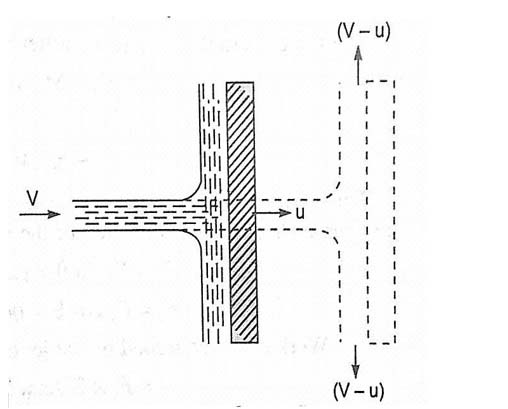
\includegraphics[width=0.5\textwidth]{img/Thrust_on_moving_flat_plate_normal_to_the_direction_of_jet.jpg}
  \caption{Thrust on moving flat plate normal to the direction of jet}
  \label{fig:Thrust_on_moving_flat_plate}
\end{figure}

Let, the flat plate moves with a velocity $u$ in the direction of the jet and the velocity of jet is $v$. The effective velocity with which the jet strike the plate = $v-u$. The mass of the fluid striking the plate per second = $\rho a (v-u)$, where $a$ is the area of the jet. \\
Thrust exerted on the plate in the direction of the jet is, 
\begin{align*}
  F &= \rho a (v-u) [(v-u) - 0]
  % F &= \rho a (v-u)^2
\end{align*}
\begin{equation}
    F = \rho a (v-u)^2 \label{eq:eq15}
\end{equation}

\begin{equation}
    \text{work done per second} = F \times u = \rho a (v-u)^{2} \times u \label{eq:eq16}
\end{equation}

However, this is not practically feasible, because the distance between the nozzle at the plate is go on increasing. If a series of plates were so arranged that each plate appeared successively before the jet in the same position and always moving with a velocity $u$ to the direction of the jet. Then mass of the fluid striking the plate = $\rho a v$.

*note : \textcolor{red}{ [ The whole flow of the nozzle is utilized by the plate. ]}

\begin{figure}[H]
  \centering
  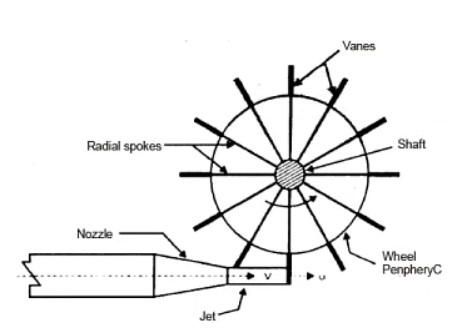
\includegraphics[width=0.5\textwidth]{img/radial_plate.jpg} 
  \caption{Thrust on Successive moving plat normal to the direction of jet}
  \label{fig:Successive_moving_plate}
\end{figure} 


The thrust on the plate,
\begin{align*}
  F &= \rho a v [(v-u) - 0] \\
  &= \rho a v (v-u)\\
\end{align*}

Work done per second = $F \times u$
\begin{equation}
  = \rho a v (v-u) u \label{eq:eq17}
\end{equation}

\begin{align*}
  \text{Now, the input power} &= \text{K.E. of the jet} \\
  &= \frac{1}{2} m v^2 \\
  &= \frac{1}{2} \rho a v \times v^2 
\end{align*}
\begin{equation}
  \therefore \text{Input power} = \frac{1}{2} \rho a v^3 \label{eq:eq18}
\end{equation}

The efficiency of the the wheel,
$$\eta = \frac{\rho a v (v-u) u}{\frac{1}{2} \rho a v^3}$$
\begin{equation}
  \eta = \frac{2u (v-u)}{v^2} \label{eq:eq19}
\end{equation}

\checkmark Generally $u$ is changed, $v$ is not changed significantly.\\

For a given jet velocity, efficiency will be maximum, if,


\begin{align*}
  \frac{d\eta}{du} &= 0 \\
  \frac{d}{du} \left[\frac{2u(v-u)}{v^2}\right] &= 0 \\
  2v - 4u &= 0 \\
  u &= \frac{v}{2}
\end{align*}

For the maximum efficiency of wheel, the peripheral speed of the wheel is equal to half of the jet velocity. \\

The max efficiency is given by - 
$$\eta_{max} = \frac{2 \frac{v}{2} (v - \frac{v}{2})}{v^2} = \frac{1}{2} = 50\% $$

\subsection{Fluid Jet (on curved plate)}
\subsubsection*{(a) stationary plate}

Velocity of jet at inlet in $x$-direction = $v_1 cos \alpha_1$ \\
Velocity of jet at outlet in $x$-direction = $v_2 cos \alpha_2$\\

Force exerted on the plate,
\begin{equation}
  F_x = \rho Q (v_1 cos \alpha_1 - v_2 cos \alpha_2) \label{ex:eq20}
\end{equation}
here, $Q = a v$   \\

If the curvature of plate at outlet such that outlet angle $\alpha_2$ is more than 90°, then the second term of the $eq^n$ (20) will be negligible. Hence in order to get more force, the curvature of the plate should be such that the angle $\alpha_2$ is obtuse.  

\subsubsection*{Single Moving Plate / Curved Vane}
\begin{figure}[H]
  \centering
  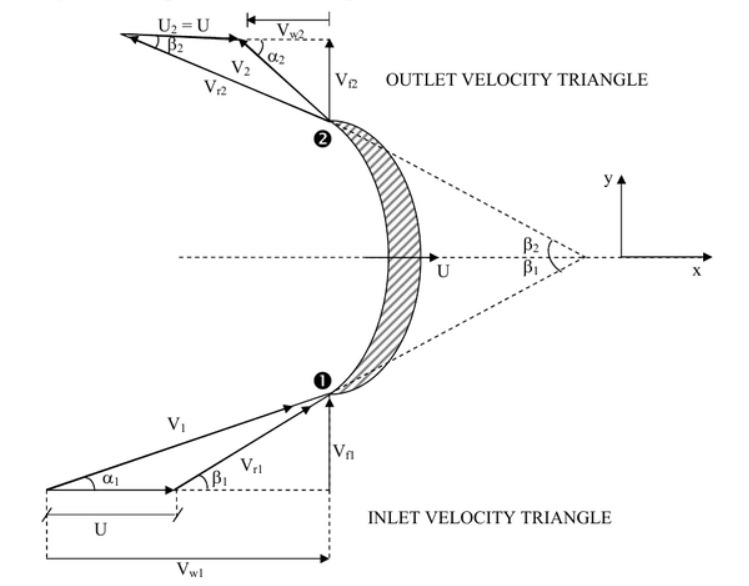
\includegraphics[width=0.8\textwidth]{img/curved_vane.jpeg} 
  \caption{Single moving plate / curved vane}
  \label{fig:curved_vane}
\end{figure} 

\begin{itemize}
  \item $v_1. v_2 \rightarrow $ Absolite velocities of the jet at inlet and outlet respectively
  \item $u_1, u_2 \rightarrow $ peripheral velocity of the vane at inlet and outlet respectively
  \item $v_{r1},v_{r2} \rightarrow $ relative velocity in inlet and outlet respectively.\\

  \begin{minipage}{0.20\textwidth}
    \begin{tcolorbox}[boxrule=1pt,width=\linewidth]
    $u + v_r = v$ \\
    $\Rightarrow v_r = v - u$ 
    \end{tcolorbox}
  \end{minipage}
  \begin{minipage}{0.33\textwidth}
    \begin{tcolorbox}[boxrule=1pt,width=\linewidth]
    $v_w, v_f$ is the components of $v$
    \end{tcolorbox}
  \end{minipage}

  \item $v_{f1}, v_{f2} \rightarrow $ velocity of flow at inlet and outlet respectively. alternatively, components of absolute velocity normal to the direction of motion.
  \item $v_{w1}, v_{w2} \rightarrow $ velocity of whirl at the inlet and outlet respectively. alternatively, components of absolute velocity in the direction of motion.  
\end{itemize}

\section{Lecture 4: Curved Vane}
\hfill Date: 17/06/2023

\subsection{Analysis of Curved Vane}
The jet enters the vane without shock if the relative $v_{r_1}$ makes an angle $\beta_1$ with the direction of motion (on x-axis). The jet glides over the vane and leaves with a velocity $v_{r_2}$. If the vane is smooth, then $v_{r_1} = v_{r_2}$. the jet will leave the vane without shock if the relative velocity $v_{r_1}$ makes an angle in $\beta_2$. \\

The mass flow rate of fluid = $\rho Q = \rho a v_r$ , where a $\rightarrow$ area of jet. 

\begin{itemize}
  \item Note: if there is only single vane, then relative velocity $v_r$ have to consider, otherwise total velocity $v$ will be counted. 
\end{itemize}

Force on the vane in the direction of motion , if $\alpha_2  < 90$°,
$$F_x = \rho a v_{r_1} \left[v_{w_1} - \left(-v_{w_2}\right)\right]$$
\begin{equation}
  F_x = \rho a v_{r_1} \left(v_{w_1} + v_{w_2}\right) \label{eq:eq21}
\end{equation}
if $\alpha_2  > 90$°, 
\begin{equation}
  F_x = \rho a v_{r_1} \left(v_{w_1} - v_{w_2}\right) \label{eq:eq22}
\end{equation}

if $\alpha_2  = 90$°, 
\begin{equation}
  F_x = \rho a v_{r_1} \left(v_{w_1} \right) \label{eq:eq23}
\end{equation}

This is the general expression of the thrust - 
$$F_x = \rho a v_{r_1} \left[v_{w_1} \pm  v_{w_2}\right]$$

if $u_1=u_2=u$, work done per second = $F_x \times u$
\begin{equation}
  = \rho a v_{r_1} \left[v_{w_1} \pm  v_{w_2}\right] \times u  \label{eq:eq24}
\end{equation}

Also work done can be determined for the changing kinetic energy. Thus the work done per second
\begin{equation}
  \text{Thus the work done per second} = \frac{1}{2} \rho a v_{r_1} \left[v_1^2 - v_2^2\right]  \label{eq:eq25}
\end{equation}

From the equation (24) \& (25),
\begin{equation}
  2(v_{w_1} \pm v_{w_2}) u = v_1^2 - v_2^2 \label{eq:eq26}
\end{equation}

Input energy of jet at inlet = $\frac{1}{2} \rho a v_1 \times v_1^2 $

The hydraulic efficiency, $$\eta = \frac{\rho a v_{r_1}  \left[v_{w_1} \pm  v_{w_2}\right] u}{\frac{1}{2} \rho a v_1 \times v_1^2}$$
\begin{equation}
  \eta = \frac{2 u v_{r_1}  \left[v_{w_1} \pm  v_{w_2}\right]}{v_1^3}  \label{eq:eq27}
\end{equation}
\pagebreak

\section{Lecture 5: Series of Vanes}
\hfill Date: 19/06/2023
If a series of vanes is fixed radially to the rim of a wheel, there is always one vane or another facing the jet. Thus the entire fluid is utilized. This arrangement of vanes is used in radial flow turbines.\\

Two types of radial flow turbine: 
\begin{enumerate}
  \item Inward flow turbine : If jet enters outer periphery
  \item Outward flow turbine : If jet enters inner periphery
\end{enumerate}

Let $R_1$ and $R_2$ be the radii of the wheel at the inlet and outlet.

\begin{figure}[h]
  \begin{center}
  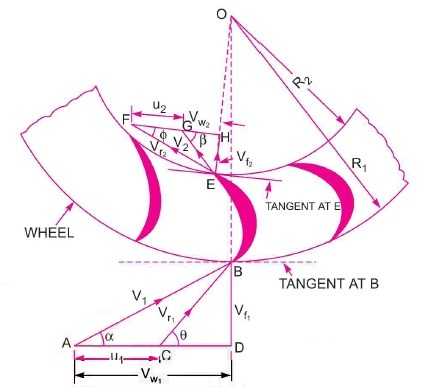
\includegraphics[width=0.8\linewidth]{img/series_vane.jpg}
    \caption{Series of vanes}
\end{center}
\end{figure}

Let, $\omega$ is the angular velocity of the wheel,
$$u_1 = \omega R_1 = \frac{2 \pi N}{60} R_1$$
$$u_2 = \omega R_2 = \frac{2 \pi N}{60} R_2$$
here, N = RPM \\
Let $m$ be the mass flow rate striking the vane. The momentum in the tangential direction at the inlet = $mv_w$ \\
The moment of momentum about the center at inlet = $mv_{w_1}R_1$\\
The moment of momentum about the center at outlet = $-mv_{w_2}R_2$\\
$\therefore$ Torque on the wheel,
$$T = mv_{w_1}R_1 - \left(-mv_{w_2}R_2\right)$$
\begin{equation}
  T = m \left(v_{w_1}R_1 + v_{w_2}R_2\right) \label{eq:eq28}
\end{equation}

\begin{align*}
  \text{Work done per second} &= T \times \omega \\
  &= m \left(v_{w_1}R_1 + v_{w_2}R_2\right) \times \omega \\ 
\end{align*}
\begin{equation}
  \text{work done per second} = m \left(v_{w_1}u_1 + v_{w_2}u_2\right)  \label{eq:eq29}
\end{equation}
Here, $\beta<$  90° \\


If $\beta>$  90°,  
\begin{equation}
  \text{work done per second} = m \left(v_{w_1}u_1 - v_{w_2}u_2\right)  \label{eq:eq30}
\end{equation}

The general expression,  
\begin{equation}
  \text{work done per second} = m \left(v_{w_1}u_1 \pm v_{w_2}u_2\right)  \label{eq:eq31}
\end{equation}
\text{This equation is known as Euler Pump Turbine equation.}

Hydraulic Efficiency,
\begin{equation}
  \eta_h = \frac{m\left(v_{w_1} u_1 \pm v_{w_2} u_2\right)}{\frac{1}{2} m v_1^2} = \frac{2\left(v_{w_1} u_1 \pm v_{w_2} u_2\right)}{v_1^2}
  \label{eq:eq32}
\end{equation}

\subsubsection*{Problem 01}
A jet of water having a velocity of 30 $ms^{-1}$ impinging for a series of vanes mounted on the periphery of a wheel moving with a peripheral velocity of 15 $ms^{-1}$. The aboslute velocity is directed at an angle of 30° to the direction of motion of vanes. The relative velocity at outlet is 95\% of the value at inlet. The absolute velocity at exit is normal to the direction of the motion of the vane. Assuming smooth entry, find the vanes angle at inlet and outlet and the hydraulic efficiency of vane. \\
\textbf{Solution}: 

\begin{multicols}{2}
  given, \\
  $v_1$ = 30 m/s \\
  $\alpha$ = 30° \\
  $u_1$ = 15 m/s \\
  $v_{r_2} = 0.95 \times v_{r_1}$ \\
  $\beta$ = 90° [normal] \\
  so, $v_{w_2} = 0, v_{2} = v_{f_2}$ \\ 
  $\checkmark$ have to add figure in exam 
\end{multicols}

\begin{multicols}{3}
  \begin{align*}
    v_{w_1} &= v_1 \cos 30 \\
    &= 30 \cos 30 \\ 
    &= 25.98 \, m/s   
  \end{align*}

  \begin{align*}
    \tan \theta &= \frac{v_{f_1}}{v_{w_1} - u_1}\\
    \theta &= 53.8    
  \end{align*}

  \begin{align*}
    v_{r_1} &= \sqrt{\left[v_{w_1} - u_1\right]^2 + (v_{f_1})^2}\\
    &= 18.59 \, m/s   
  \end{align*}

  \begin{align*}
    v_{r_2} &= 0.95 \times v_{r_1}\\
    &= 17.67 \, m/s   
  \end{align*}

  \begin{align*}
    & \text{Assuminng } u_1 = u_2, \\
    \cos \phi &= \frac{v_{f_2}}{u_2}\\
    \phi &= \cos^{-1} \left(\frac{15}{17.66}\right) \\ 
    &= 27.53 
  \end{align*}

  \begin{align*}
    \eta_h &= \frac{2 v_{w_1} u_1}{v_1^2}\\
    \eta_h &= \frac{2 \times 25.98 \times 15}{30^2}\\
    &= 0.866 \\
    &= 86.7\%  
  \end{align*}


\end{multicols}

\subsubsection*{Problem 02}
A jet of water 5 cm in diameter inpinges on a curved vane and is deflected through an angle of 175°. The vane moves in the same direction at that of the jet with a velocity of 35 m/s. The rate of flow is 170 l/s. Determine the compounds forces, horse power developed by the vane and water efficiency. Neglect friction. Solve this problem, if instead of one vane, there are a series of vanes fixed to a wheel.\\
$F_x = ?, F_y = ? , HP = ?, \eta_h = ?$\\

\textbf{Solution:} 
\begin{multicols}{2}
  Given,\\
  d = 5 cm \\
  u = 35 m/s \\
  Q = 170 l/s = 0.17 $m^3/s$ \\
  $$v = \frac{Q}{a} = \frac{0.17}{0.196\times 10^{-2}} = 86.58 /, m/s$$ \\
  $$a = \frac{\pi}{4} \left[0.05\right]^2 = 0.196 \times 10^{-2} /, m^2$$ \\
  v= u + $v_r$ \\
  $v_r = 86.58 - 35 = 51.58$ m/s \\ 
\end{multicols}

Neglecting friction,\\
\begin{align*}
  v_{r_1} = v_r &= 51.58 \, m/s \\\
  v_{r_1} \cos \phi &= 51.38 \, m/s \\
  \therefore v_{w_1} = v_{r_1} \cos \phi - u_1 &= 51.38 -35 = 16.38 \, m/s \, [u = u_1] \\ 
\end{align*}

\begin{align*}
  F_x &=\rho a v_r \left(v_w + v_{w_1}\right) = 10427.87 N \\
  F_y &=\rho a v_r \times v_{f_1} \\
  HP &= \frac{F_x u}{746} \\
  \eta_h &= \frac{F_x u}{\frac{1}{2} m v^2} =  \frac{10427.87 \times 35}{\frac{1}{2} \times 1000 \times 0.17 \times 86.58^2} = 57.3\% 
\end{align*}
\hrulefill


\section{Lecture 6: Hydraulic Turbines}
\hfill Date: 24/06/2023

Hydraulic turbines are the machines which converts the hydraulic energy into mechanical energy. In other words, hydraulic turbines are prime movers which run with hydraulic energy. The mechanical energy produced by a hydraulic turbine can be connected into electric energy by coupling the turbine to an electric generator. 

\subsection*{Classfications of Turbines}
May be classified according to the following criteria:
\begin{enumerate}
  \item Hydraulic action 
  \item Direction of fuel of water 
  \item Direction of the shaft
  \item Head 
  \item Specific Speed 
\end{enumerate}

\subsubsection*{Prime Mover}
Prime movers refer to the mechanical devices or systems that convert hydraulic energy (the energy of flowing or falling water) into mechanical energy (rotational motion). These prime movers are responsible for driving the turbine rotor and generating power. In the case of hydraulic turbines, the most common type of prime mover is an electric generator or alternator. The turbine is connected to the rotor of the generator, and as the turbine rotates, it transfers its mechanical energy to the generator, which then converts it into electrical energy. The prime mover can also be a mechanical drive system, such as a gearbox or a shaft, which is connected to various industrial machines or equipment. In such cases, the mechanical energy produced by the turbine is directly transmitted to the driven machinery to perform specific tasks. The choice of prime mover depends on the application and the desired output. In most large-scale hydropower plants, electric generators are used as prime movers to produce electrical power that can be transmitted over long distances and distributed to consumers. In other industrial applications, mechanical prime movers may be employed for specific operations within a facility.

\subsubsection*{Specific Speed}
The specific speed of a hydraulic turbine is a dimensionless parameter that characterizes the geometric and hydraulic performance of the turbine. Specific speed (Ns) is defined as the speed at which a geometrically similar turbine would operate to produce unit power (1 horsepower or 1 kilowatt) under a unit head (1 foot or 1 meter).

\subsection*{Hydraulic Action}
\begin{enumerate}
  \item \textbf{Impulse Turbine:} Here the available head is converted into kinetic energy by passing the water through a nozzles. Ex - Pelton wheel, girard turbine, banki turbine etc. 
  \item \textbf{Reaction Turbine:} A part of the total head is connected in kinetic energy and the rest remains in the form of pressure energy. Example of reaction turbines - kaplan turbine, propeller turbine, etc. 

\end{enumerate}

\subsection*{Direction of flow of water}
\begin{enumerate}
  \item Tangent flow turbine : The water strikes the runner in the direction of tangent to the wheel. Ex - pelton wheel. 
  \item radial flow turbine: may be classified as inward flow and outward flow. Ex - francis turbine (old) (inward flow)
  \item Axial Flow : Kaplan and propeller turbine 
  \item Mixed Flow Turbine : Francis turbine 
\end{enumerate}

\subsection*{Direction of the shaft}
\begin{enumerate}
  \item Vertical : shaft vertical, runner horizontal 
  \item Horizontal : shaft horizontal, runner vertical 
\end{enumerate}

\subsection*{Head}
\begin{enumerate}
  \item High Speed Turbine: Net head is 150m - 2000 m. Ex - pelton wheel turbine 
  \item Medium Head Turbine: Head from 30 m - 150 m. Ex - Francis Turbine 
  \item Tow Head Turbine: Head < 30 m. Ex - Kaplan and propeller. (kaptai)  
\end{enumerate}

\subsection*{Specific speed}
\begin{enumerate}
  \item Low Specific Speed : speed < 60. Ex - pelton wheel 
  \item Medium Specific Speed : 60 < speed < 400.  Ex - Francis turbine. 
  \item High Specific Speed: speed > 400. Ex - Kaplan Turbine. 
\end{enumerate}

\subsection*{Difference between axial and radial hydraulic turbine }
\begin{itemize}
  \item Fluid Flow Direction:

  \textbf{Axial Hydraulic Turbine}: In an axial hydraulic turbine, the water flow is parallel to the axis of rotation. The water enters the turbine axially and passes through the rotor blades in the same axial direction.\\

  \textbf{Radial Hydraulic Turbine}: In a radial hydraulic turbine, the water flow is radial, moving inward or outward from the center of the turbine. The water enters the turbine radially and flows through the rotor blades in a radial direction.
  \item Blade Orientation and Configuration:
  
  \textbf{Axial Hydraulic Turbine}: Axial turbines have rotor blades arranged in a propeller-like configuration, similar to the blades of a ship's propeller. The blades are oriented parallel to the axis of rotation and typically have a streamlined shape to efficiently capture the water's energy.\\

  \textbf{Radial Hydraulic Turbine}: Radial turbines have rotor blades arranged in a radial pattern, perpendicular to the axis of rotation. The blades extend radially from the center of the turbine and are typically straight or slightly curved. They are designed to effectively capture the water flow in a radial direction.
  \item Applications:
  
   \textbf{Axial Hydraulic Turbine}: Axial turbines are commonly used in high-flow, low-head applications, such as in large-scale hydropower plants. They are suitable for situations where a large volume of water needs to be harnessed efficiently.\\

  \textbf{Radial Hydraulic Turbine}: Radial turbines are typically employed in low-flow, high-head applications. They are often used in small-scale hydropower installations, such as run-of-river projects or micro-hydropower systems.

  \item Efficiency and Performance:
  
  \textbf{Axial Hydraulic Turbine}: Axial turbines are known for their high efficiency at high flow rates. They can handle a significant volume of water and are well-suited for sites with a substantial water supply.\\

  \textbf{Radial Hydraulic Turbine}: Radial turbines are efficient in applications where there is a significant pressure drop. They are designed to generate power under high head conditions, where water is available at a relatively low flow rate.
\end{itemize}
\hrule
\end{document}
